{\bf{В первой}} главе ставится и решается задача разработки алгоритма оценки информационных параметров CDMA-систем на фоне аддитивного белого гауссового шума.

Математическую модель входной смеси CDMA-сигнала с двоичной фазовой модуляцией на приемной стороне может быть представлена как:
\begin{equation}
	\label{eq:cdma_eq}
	x(t)=\sum\limits_{k=1}^{N}A_k d_k(t)g_k(t)\cos{(\omega_{k}t + \phi_k(t))} + n(t)
\end{equation}
где ${A_k}$ - амплитуда несущей, ${d_k}(t)$ - информационная последовательность, ${g_k}(t)$ - ПСП последовательность, ${\phi_k(t)}$ - фаза, обусловленная допплеровским смещением частоты, 
${n(t)}$ - шумовая компонента. Информационная последовательность ${d_k}(t)$ и ПСП последовательность ${g_k}(t)$ представляют собой потоки антиподных импульсов.

После оцифровки и повторного модулирования входной смеси (\ref{eq:cdma_eq}), содержащей один источник информации, с ПСП в данном случае получается:
\begin{equation}
	\label{eq:cdma_strip_eq}
	x_k(m) = A_k \cos{(\tilde{\omega}_{k}m + \phi_k(m))} + n_k(m)
\end{equation}
где ${m}$ - индекс соответствующий времени, ${\tilde{\omega}_k}$ - нормированная частота, соответствующая ${\omega_k}$, ${n_k}(m)$ - шум ${n(t)}$, умноженный на ПСП.

Для восстановления гармонического сигнала входную смесь необходимо повторно модулировать ПСП с учетом правильной оценки фазы ПСП.
В реальных условиях приемник не имеет информации о фазе ПСП поэтому для оценки промежуточной частоты 
сигнала необходимо перебрать все возможные значения фазы ПСП. Для снижения вычислительных затрат предлагается использование алгоритма быстрого преобразования Фурье (БПФ).
Схема алгоритма представлена на Рис. \ref{pic:ar_cdma1_scheme2}.
\begin{figure}[h]
	\center\scalebox{0.9}{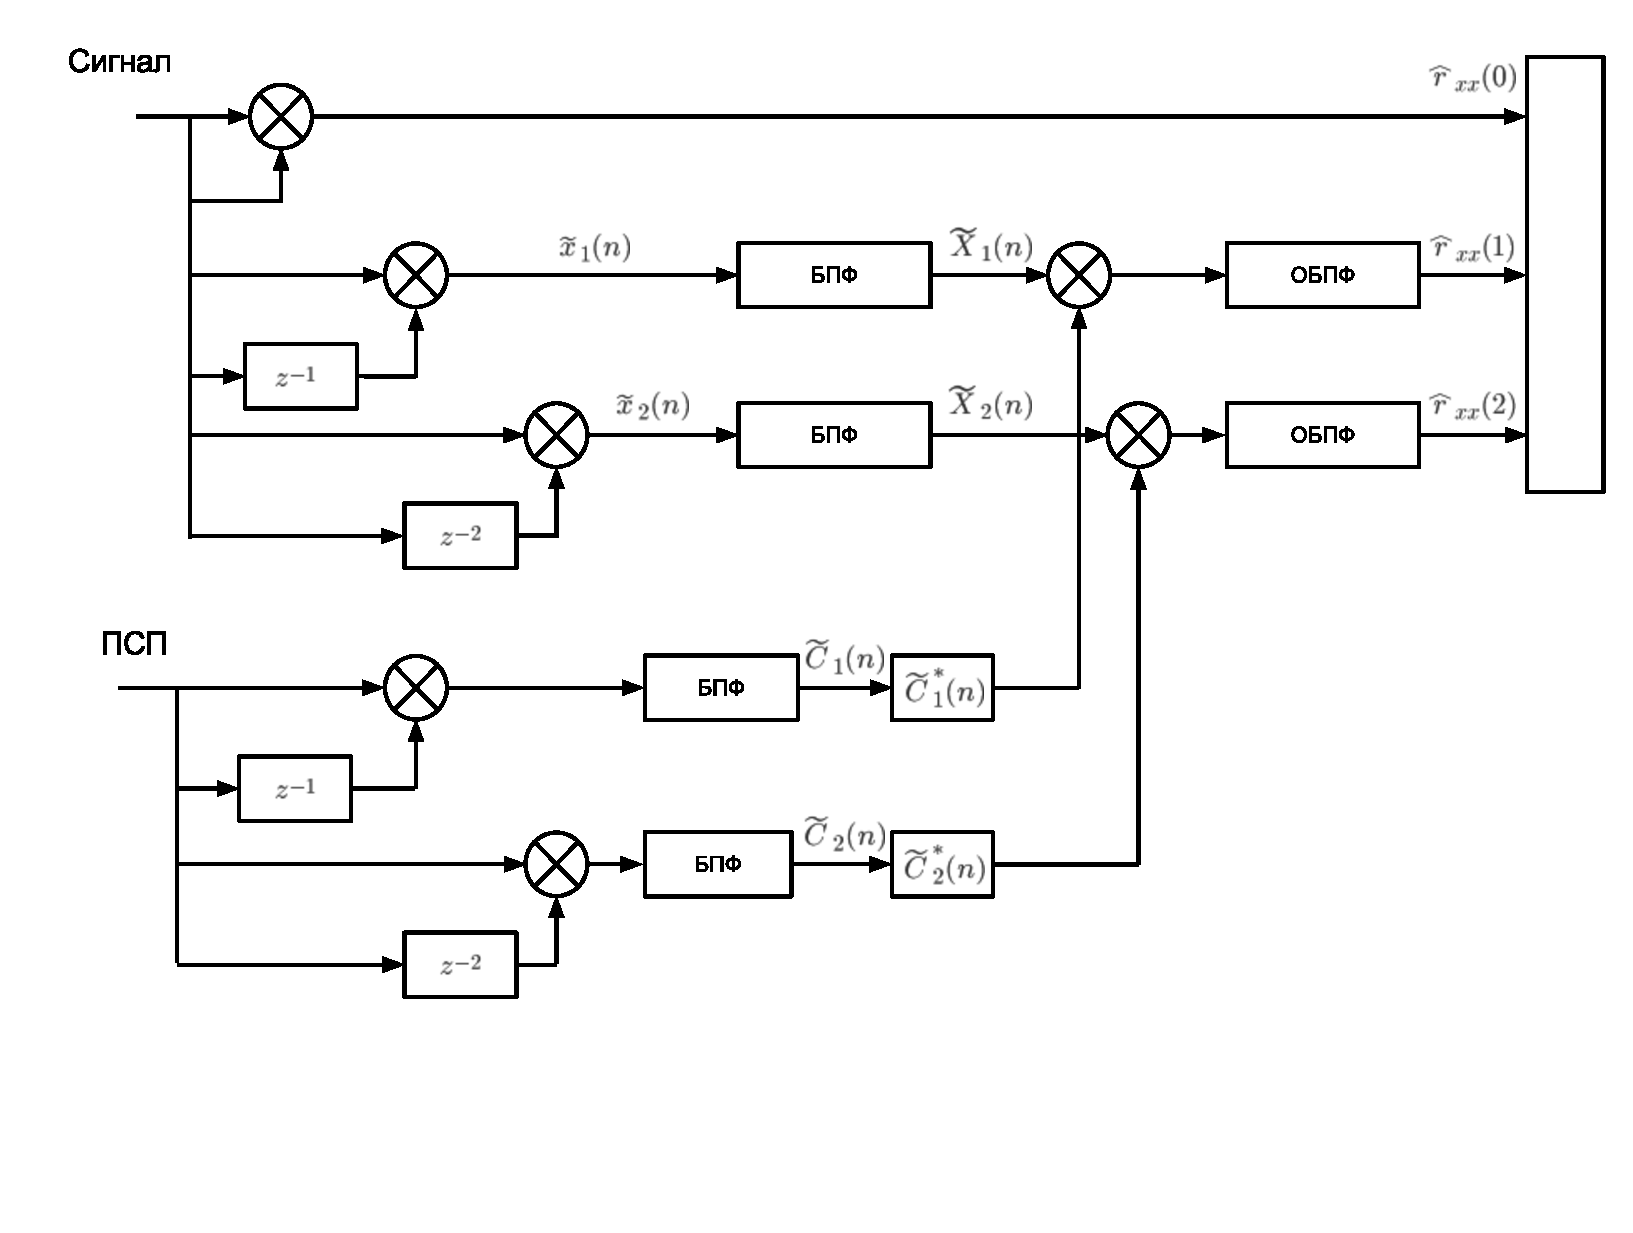
\includegraphics[width=1\linewidth]{lpc_fft.eps}}
	\caption{Общая схема применения АР модели для детектирования ШПС сигнала.}
	\label{pic:ar_cdma1_scheme2}
\end{figure}

Оценка ${\hat{r}_{xx}(0)}$ не зависит от выбранной фазы ПСП, поэтому она вычисляется один
раз для всех смещений кода. Далее формируется массив произведений входной смеси на
свою задержанную копию ${\tilde{x}_1(m)=x(m)x(n-1)}$. Полученная последовательность  
${\tilde{x}_1(m)}$ поступает на вход алгоритма БПФ, в результате получаем массив ${\tilde{X}_1(m)}$
содержащий частотные отсчеты. Аналогично формируется массив  ${\tilde{X}_2(m)}$ для
задержки входного сигнала равной двум. Таким же способом обрабатываются локально
сгенерированные ПСП и формируются два массива ${\tilde{g}_1(m)}$ и ${\tilde{g}_2(m)}$.
Далее массивы ${\tilde{X}_1(m)}$ и ${\tilde{X}_1(m)}$ поэлементно перемножаются
на комплексно сопряженные массивы ${\tilde{G}_1^*(m)}$ и ${\tilde{G}_2^*(m)}$.
Результаты этих перемножений поступают на вход алгоритма обратного
БПФ (ОБПФ). Полученные после ОБПФ два массива содержат оценки автокорреляционной функции для ${N}$ 
фаз ПСП, где  ${N}$ - размер данных на входе алгоритма БПФ.

Таким образом, предлагаемый алгоритм состоит из следующих шагов:

\begin{itemize}
\item[Шаг 1.] Вычисляются оценки  АКФ в трех первых точках (для аргументов АКФ=0,1,2)
	с использованием алгоритма БПФ для всех возможных смещений ПСП. 
\item[Шаг 2.] Для каждого смещения ПСП: 
	Определяются коэффициенты АР-модели ${\hat{a_1}, \hat{a_2}}$,
	вычисляется резонансная частота ${\omega_0}$
	и определяется квадрат модуля частотного отклика АР-модели для этой частоты. 
\item[Шаг 3.] Выбирается смещение ПСП для которого значение квадрата модуля частотного отклика было максимальным. Полученное значение сравнивается с заранее выбранным порогом детектора. 
	\subitem{\underline{Если}}  значение оказалось больше порогового {\underline{то}} 
		принимается решение о наличии сигнала, а в качестве оценки
		частоты принимается значение ${\omega_0}$ соответствующее выбранному смещению ПСП. 
	\subitem{\underline{Иначе}} 
		Принимается решение об отсутствии гармонического сигнала.
\end{itemize}

Разработанный алгоритм позволяет производить оценку частоты гармонического сигнала без использования прямого перебора по частоте, как это делается в большинстве современных алгоритмов.
Например, алгоритм Delay and Multiply Approach (DMA) позволяет производить поиск только по фазе ПСП, но он не дает возможности прямой оценки частоты. 
Предложенный алгоритм допускает сокращение количества операций умножения при переборе значений фазы ПСП за счет использования алгоритма БПФ.

Основным недостатком предложенного алгоритма является сильная чувствительность по отношению к интерференционным помехам - межканальной интерференции (МКИ):
наличие «окрашенного» шума в рабочей полосе приводит к значительному смещению получаемых оценок информационных параметров.

Количество операций для оценки информационных параметров от одного источника на фоне АБГШ:
\begin{equation}
	%\label{}
	OP_{AR\_FOR\_1} = 24NlogN + 63N
\end{equation}

График вероятности оценки частоты в допустимом диапазоне входной расстройки модуля фазовой автоподстройки частоты (ФАПЧ) представлен на Рис.
\ref{pic:lpc_for_1_probability}. Моделирование проводилось с аддитивным шумом, заданным в полосе от 0 Гц до
половины частоты дискретизации для одного. В данном случае значение частоты дискретизации равно 16.368 МГц.
\begin{figure}[H]
\center\scalebox{1}{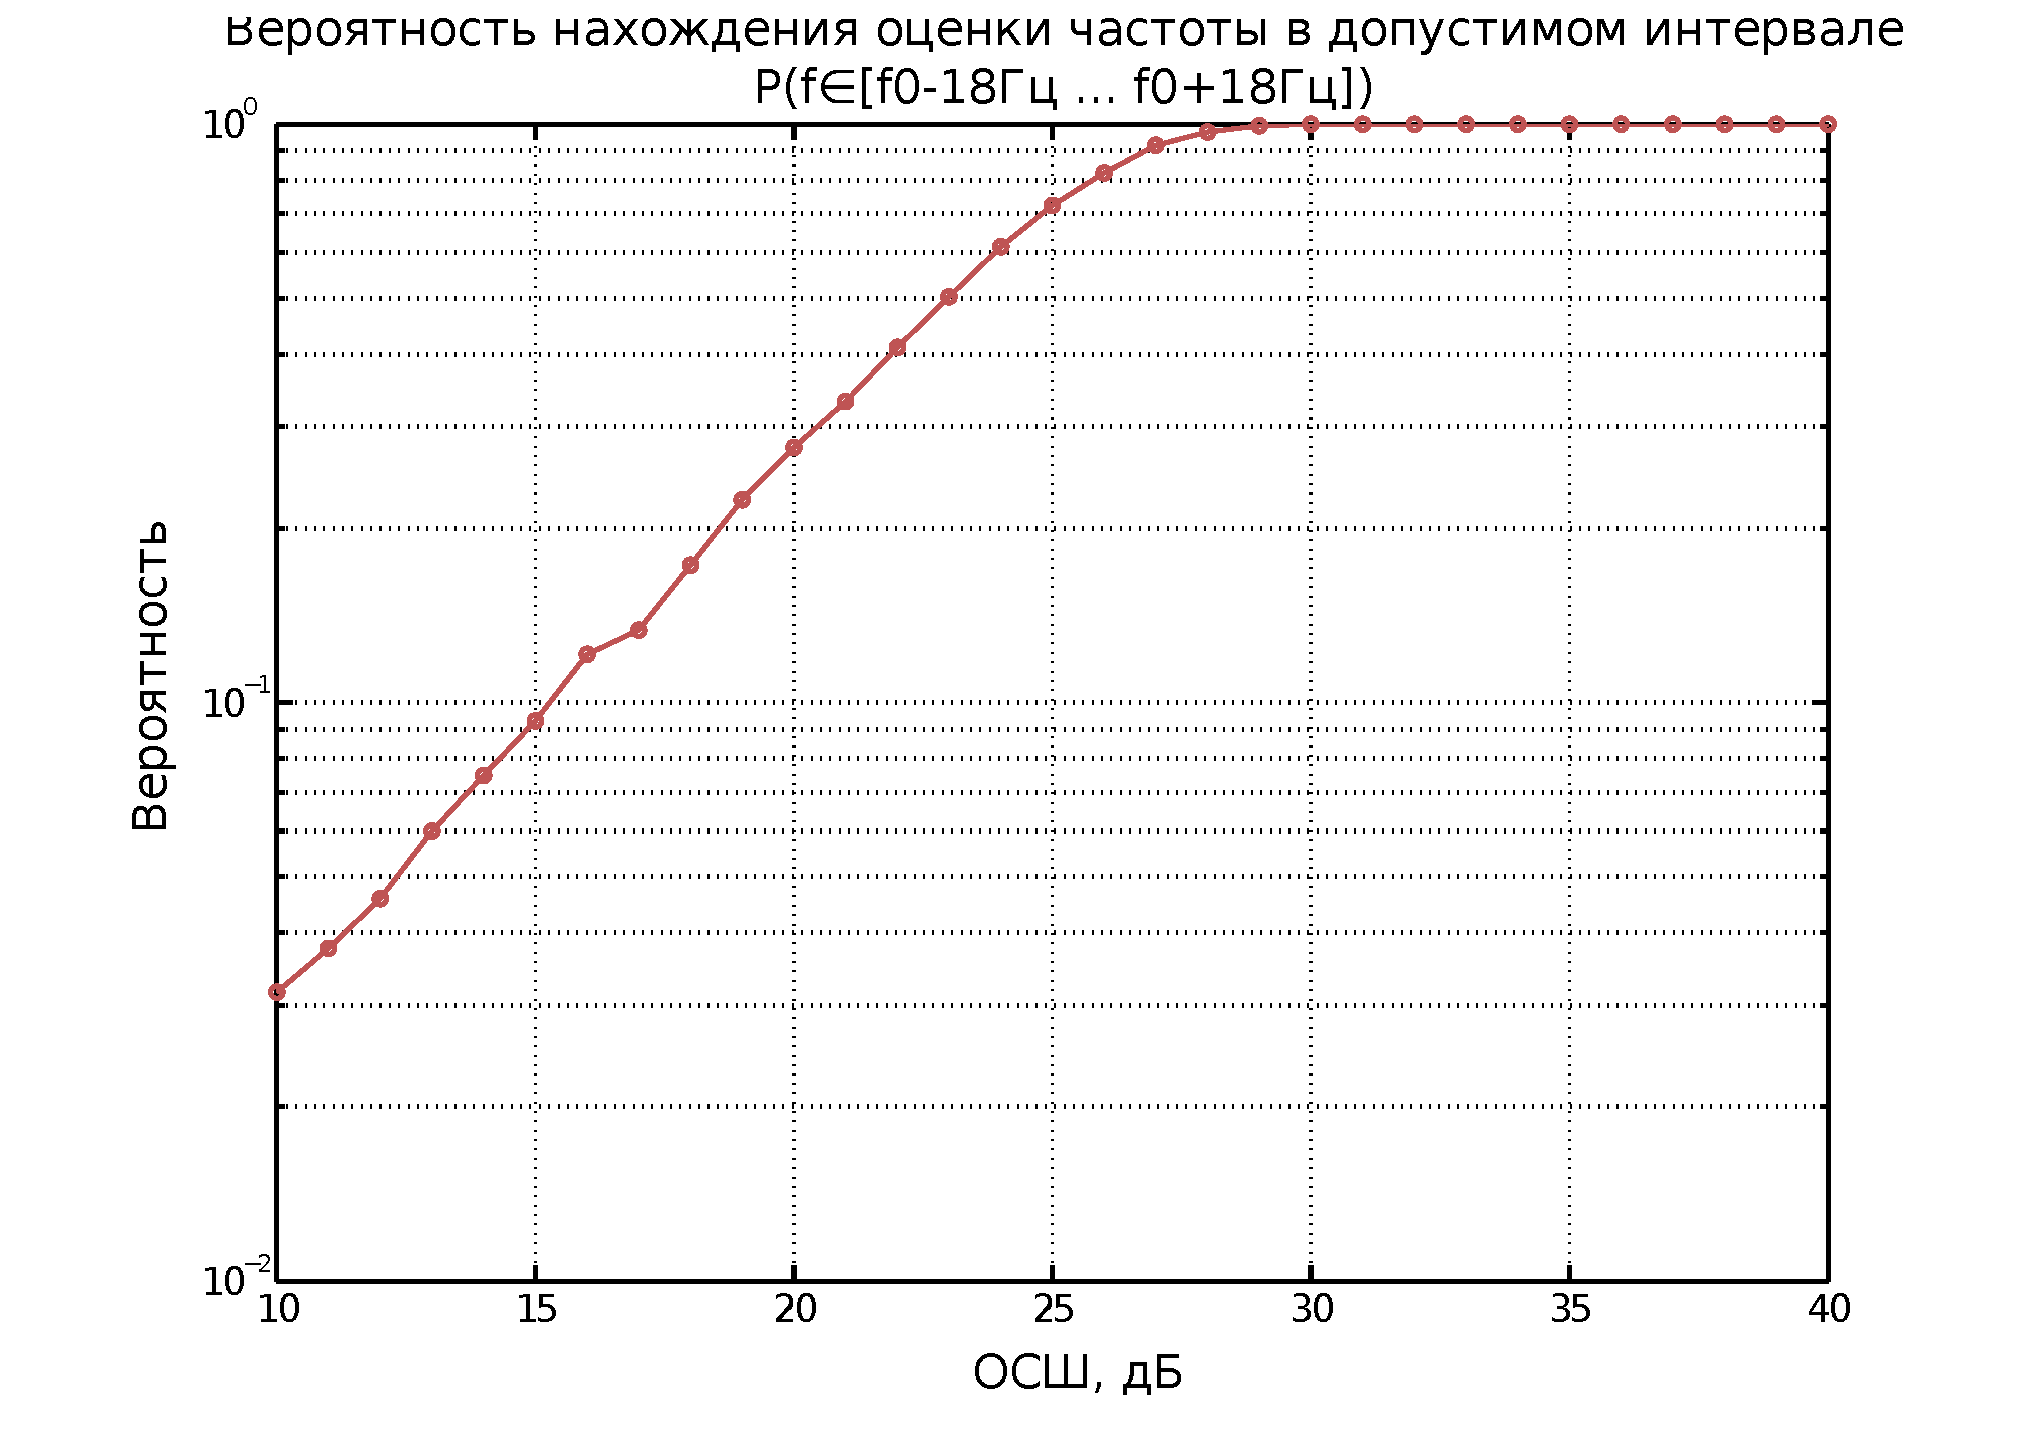
\includegraphics[width=1\linewidth]{lpc_for_1_probability.eps}}
	\caption{Вероятность оценки частоты удовлетворяющей допустимой входной расстройке ФАПЧ}
	\label{pic:lpc_for_1_probability}
\end{figure}

Для оценки точности можно сравнить предлагаемый алгоритм с границей Крамера-Рао (КР). Неравенство Крамера-Рао дает базу оценки, так
как представляет минимальную дисперсию оцениваемой величины среди всех классов оценщиков.
\begin{figure}[H]
\center\scalebox{1}{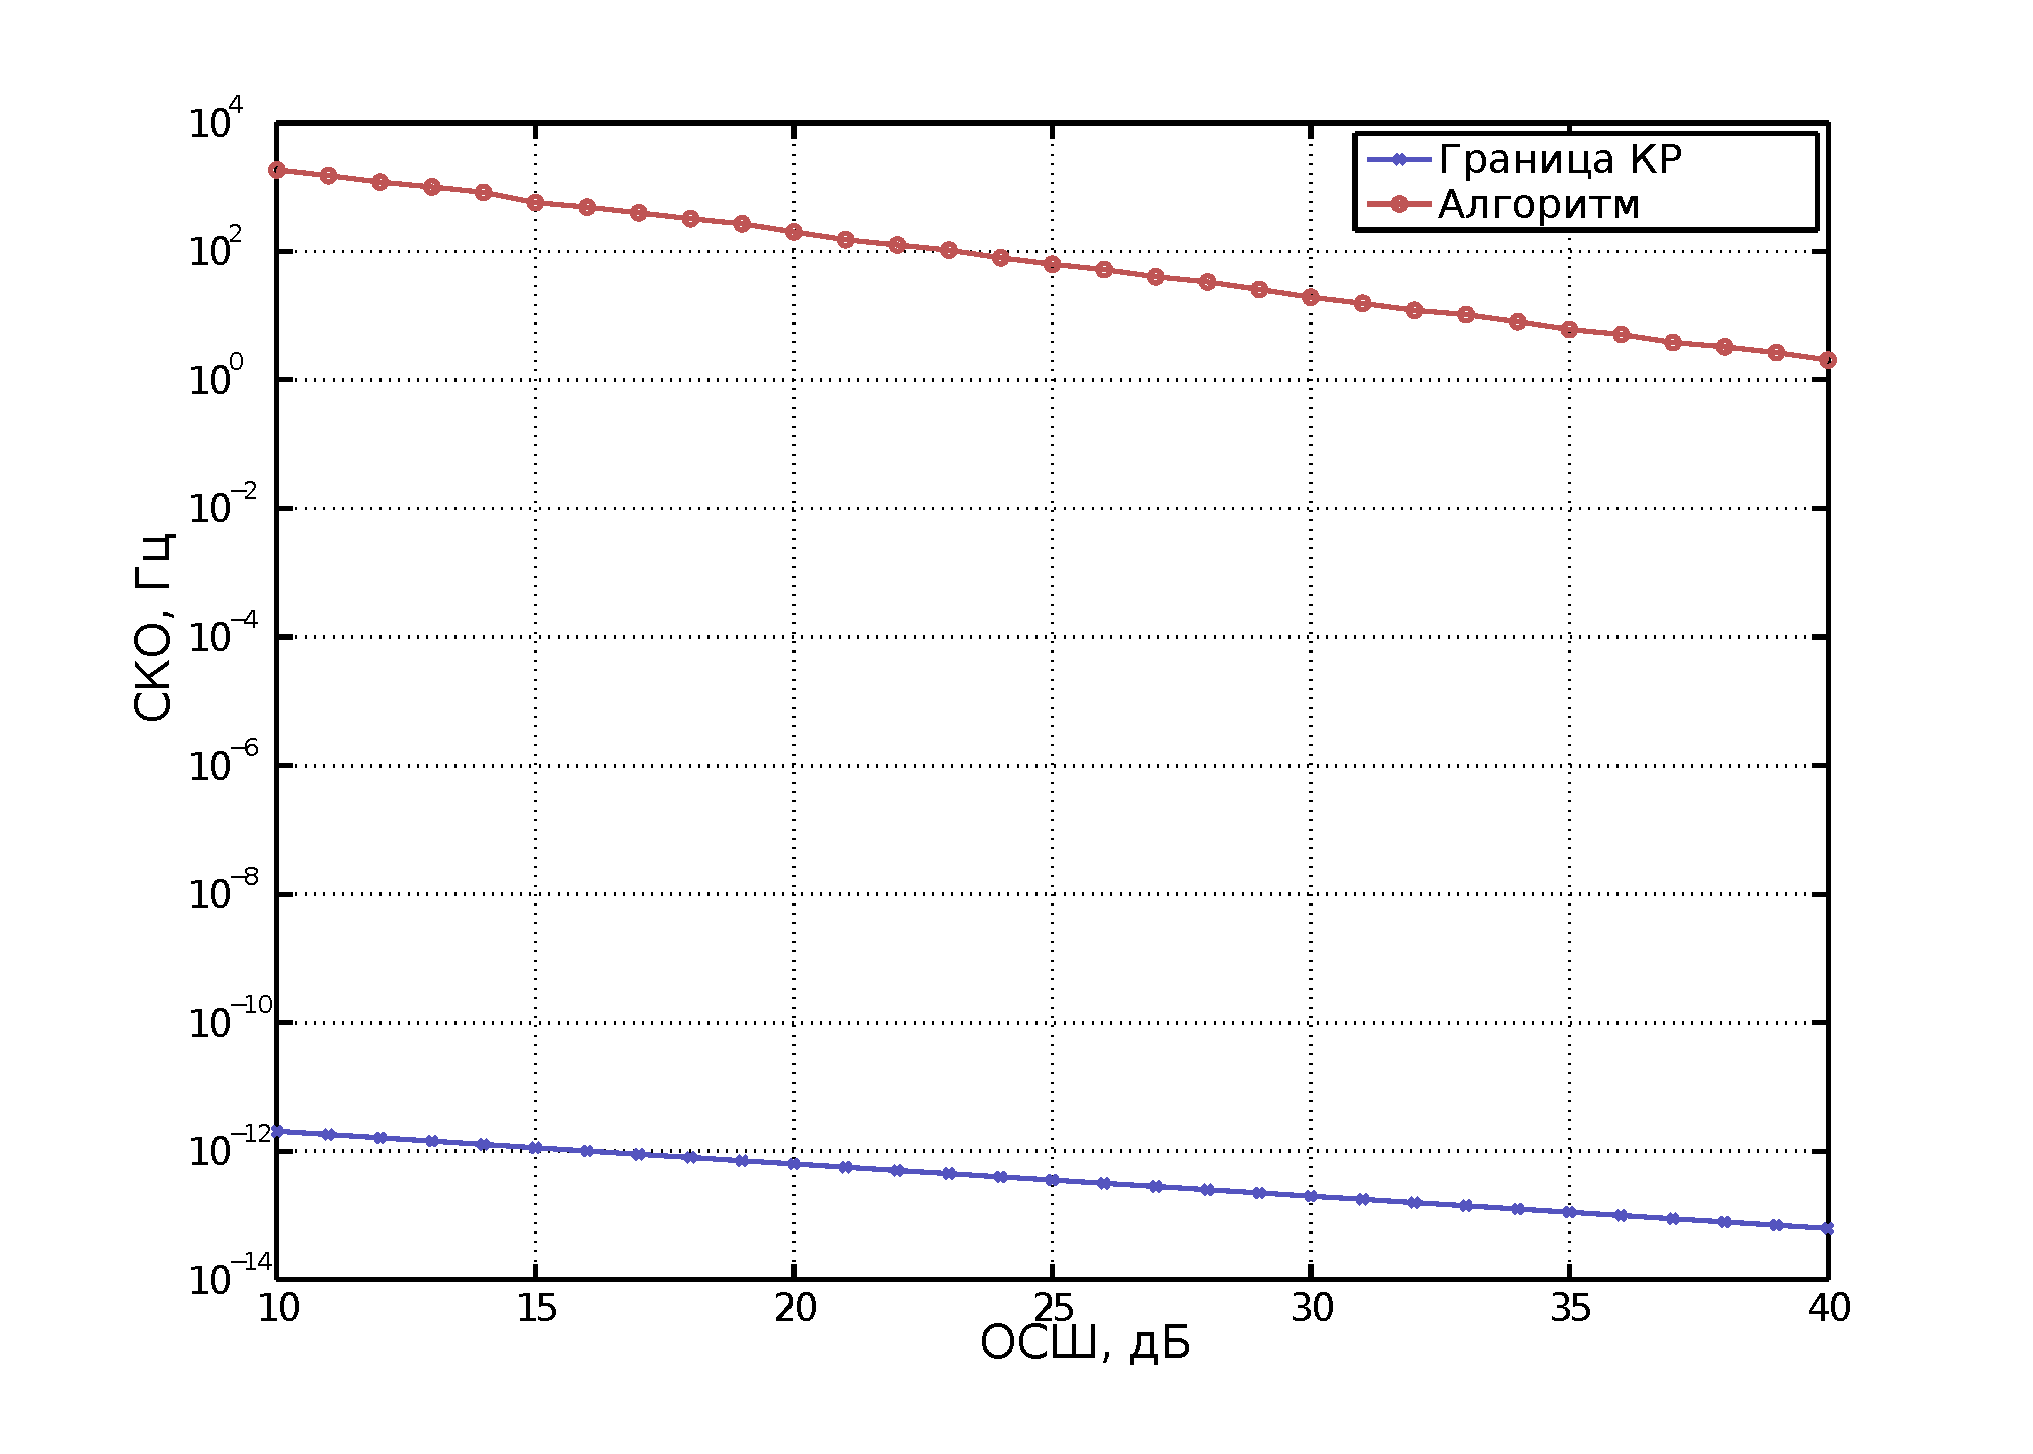
\includegraphics[width=1\linewidth]{crlb_vs_1sat_algo.eps}}
	\caption{СКО ошибки оценки частоты}
	\label{pic:crlb_vs_1sat_algo}
\end{figure}
